\clearpage
\appendix
\renewcommand{\thesubsection}{\thesection\arabic{subsection}}
\refstepcounter{section}
\section*{Appendix \thesection}
\markboth{Appendix \thesection}{Appendix \thesection}
\addcontentsline{toc}{section}{Appendix \thesection}
\label{app:additional_material}

% Number appendix floats with the appendix letter (Table A1, Figure A1, ...)
\renewcommand{\thetable}{\thesection\arabic{table}}
\renewcommand{\thefigure}{\thesection\arabic{figure}}
\setcounter{table}{0}
\setcounter{figure}{0}

\subsection{Data Availability and Operational Timing}
\label{app:data_timing}

Table~\ref{tab:data_timing} documents the main availability times shown in
Figure~\ref{fig:operational_timeline}. Regulatory deadlines and exchange rules
are binding latest times. Platform behavior and publication latencies describe
typical availability and can deviate on individual days. The admissible
information set of Section~\ref{sec:operational_information_set} is applied
with these availability times at every cutoff.

\begin{table}[H]
  \centering
  \footnotesize
  \caption[Data sources and availability times of the operational inputs.]
  {Sources and status of the operational availability times used in
  Figure~\ref{fig:operational_timeline}.}
  \label{tab:data_timing}
  \begin{tabular}{@{}>{\raggedright\arraybackslash}p{0.26\textwidth}
                  >{\raggedright\arraybackslash}p{0.34\textwidth}
                  >{\raggedright\arraybackslash}p{0.32\textwidth}@{}}
    \toprule
    Element & Operational timing used & Source and status \\
    \midrule
    SDAC gate closure
    & 12:00 on day \(d-1\)
    & Exchange rule \cite{epexSpotPowerMarket} \\
    \addlinespace
    \mbox{ENTSO-E} day-ahead load forecast
    & Regulatory deadline two hours before gate closure, observed available
      around 10:30 on day \(d-1\) in the data collection
    & Regulatory deadline, Regulation 543/2013 Art.~6(1)(b)
      \cite{euRegulation543_2013}, availability observed by the data
      collection \\
    \addlinespace
    \mbox{ENTSO-E} realized load
    & Published no later than one hour after the operating period
    & Regulatory deadline, Art.~6(1)(a) \cite{euRegulation543_2013} \\
    \addlinespace
    \mbox{ENTSO-E} realized wind and solar generation
    & Published no later than one hour after the operating period, with
      initial estimates updated as measured data becomes available
    & Regulatory deadline, Art.~16(1)(j) \cite{euRegulation543_2013} \\
    \addlinespace
    \mbox{ENTSO-E} day-ahead wind and solar forecast
    & Published after the 12:00 gate closure and no later than
      18:00 on day \(d-1\)
    & Publication time reported for the \mbox{ENTSO-E} Transparency Platform
      \cite{kleinebrahm2026energyarena}, with the publication requirement set
      under Art.~14(2)(d) \cite{euRegulation543_2013} \\
    \addlinespace
    EXAA day-ahead prices
    & Auction closes at 10:15 on day \(d-1\). EXAA
      day-ahead prices for Germany are published on the \mbox{ENTSO-E} Transparency
      Platform around 11:15
    & Exchange rule \cite{exaaTradingRules2025}, publication time
      \cite{entsoeTransparency,eiser2026operational} \\
    \addlinespace
    Control-reserve auction results
    & German control-reserve capacity auctions for delivery day \(d\) close on
      day \(d-1\) at 08:00 (FCR), 09:00 (aFRR), and 10:00 (mFRR). Their
      results are used from one hour after gate closure. A check on
      28~September~2026 found them published 14 to 23 minutes after gate
      closure
    & Auction platform \cite{regelleistungNet2026} \\
    \addlinespace
    SDAC auction results
    & Released after gate closure and therefore not admissible before
      12:00
    & Market-coupling process \cite{epexSpotMarketCoupling} \\
    \addlinespace
    \mbox{ICON-D2} weather forecasts
    & A new run starts every three hours and is complete about 80 minutes after
      its start
    & DWD Open Data \cite{dwdIconForecastData} and Open-Meteo documentation
      \cite{openMeteoForecastApi} \\
    \bottomrule
  \end{tabular}
\end{table}

\FloatBarrier

\subsection{Model Configurations}
\label{app:model_configs}

Table~\ref{tab:model_configs} summarizes the final configuration of every model
in the pipeline. All models use a rolling origin: for each delivery day they are
refitted on a trailing training window ending on the day before delivery. The
load, solar, and wind forecasting models use their own task-specific weather
representations and forecast creation times, while the price models use the
coarse two-cluster weather aggregation selected on the development period
(Appendix~\ref{app:price_base_selection}). The RQ3 cutoff models reuse the RQ2
price-model configuration and vary only the admissible information set with the
forecast creation time.

\begin{table}[H]
  \centering
  \footnotesize
  \setlength{\tabcolsep}{3.8pt}
  \caption[Final model configurations.]
  {Final configuration of each pipeline model. The window is the length of the
  rolling training window in days. All weather features are derived from the DWD
  ICON-D2 model, accessed through DWD Open Data or the Open-Meteo API.}
  \label{tab:model_configs}
  \begin{tabular}{@{}>{\raggedright\arraybackslash}p{0.135\textwidth}
                  >{\raggedright\arraybackslash}p{0.11\textwidth}
                  >{\raggedright\arraybackslash}p{0.055\textwidth}
                  >{\raggedright\arraybackslash}p{0.20\textwidth}
                  >{\raggedright\arraybackslash}p{0.27\textwidth}@{}}
    \toprule
    Model & Estimator & Win. & Weather representation & Key inputs \\
    \midrule
    Load, correction
      & LightGBM & 224 & \mbox{ICON-D2}, 25 clusters, population-weighted
      & \mbox{ENTSO-E} load forecast, realized load to 10:30, calendar, weather \\
    \addlinespace
    Load, direct
      & LightGBM & 224 & \mbox{ICON-D2}, 25 clusters, population-weighted
      & Realized load to the cutoff, calendar, and weather, without the
        \mbox{ENTSO-E} forecast \\
    \addlinespace
    Solar
      & Hist.\ gradient boosting & 90 & \mbox{ICON-D2}, 25 clusters per TSO,
        capacity-weighted
      & Clear-sky geometry and physics baseline, irradiance, cloud cover,
        installed capacity \\
    \addlinespace
    Wind
      & Hist.\ gradient boosting & 180 & ICON-D2 incl.\ hub-height fields, 100 clusters
        incl.\ offshore, capacity-weighted
      & Hub-height wind speed, power-curve and cubic transforms, installed
        capacity \\
    \addlinespace
    Price \(\hat{P}^{\mathrm{base}}\)
      & LightGBM, 300 trees & 70 & \mbox{ICON-D2}, 2 clusters
      & Price lags, calendar, weather, \mbox{ENTSO-E} load forecast \\
    \addlinespace
    Price \(\hat{P}^{\mathrm{gen}}\)
      & LightGBM, 300 trees & 70 & \mbox{ICON-D2}, 2 clusters
      & As \(\hat{P}^{\mathrm{base}}\), with the \mbox{ENTSO-E} load forecast
        replaced by the OBTF load, renewable-generation, and residual-load
        forecasts \\
    \addlinespace
    Price, RQ3 cutoffs
      & LightGBM, 300 trees & 70 & \mbox{ICON-D2}, 2 clusters, 06~UTC run
        at all cutoffs
      & Inputs admissible at each cutoff, adding reserve-market results from
        09:00 and EXAA prices at 12:00 \\
    \bottomrule
  \end{tabular}
\end{table}

\FloatBarrier

\subsection{Additional Price Forecast Results}
\label{app:price_results}

This appendix reports the development-period selection of the base price model,
which fixes the rolling training window and the weather-cluster count used
throughout the price experiments.

\subsubsection{Selection of the Base Price Model Window and Weather Clustering}
\label{app:price_base_selection}

The rolling training window and the raw-weather cluster count of the base
price model are selected by a staged search on the development period
(20~December~2025 to 31~January~2026), so that no design choice depends on the
test period. The search is a coordinate descent. The training window is chosen
first at a fixed mid-range count of sixteen weather clusters, the boosted-tree
hyperparameters are chosen next at the selected window, and the number of
weather clusters is chosen last at the selected window. The hyperparameter stage
selects a small tree size and moderate \(L_2\) regularization, with the number of
leaves having little effect at the available sample size and stronger
regularization degrading accuracy. The two knobs that carry the comparison are
therefore the window length and the cluster count, reported below.

Table~\ref{tab:price_base_window} varies the training window from 28 days to an
expanding window that uses all post-transition history. Development-period
accuracy improves up to 70 days and then plateaus, and the expanding window
gives no meaningful further gain. A 70-day window is selected.

\begin{table}[H]
  \centering
  \small
  \caption[Base price model training-window selection.]
  {Development-period accuracy of the base price model over the rolling
  training window, at sixteen weather clusters and 300 boosted-tree rounds. The
  expanding window uses all post-transition history. The selected window is in
  bold. Errors are in EUR/MWh.}
  \label{tab:price_base_window}
  \begin{tabular}{@{}lrr@{}}
    \toprule
    Training window (days) & RMSE & MAE \\
    \midrule
    28        & 26.75 & 16.79 \\
    42        & 26.37 & 16.36 \\
    56        & 24.49 & 14.75 \\
    \textbf{70} & \textbf{23.30} & \textbf{14.19} \\
    Expanding & 23.21 & 14.28 \\
    \bottomrule
  \end{tabular}
\end{table}

Table~\ref{tab:price_base_clusters} fixes the window at 70 days and varies the
number of weather clusters from 1 to 100. Accuracy is best at two clusters and
degrades as the spatial resolution increases, while the mean training time per
delivery day grows from about twelve seconds at one cluster to nearly half an
hour at one hundred clusters. Finer spatial resolution therefore raises the
training cost sharply without improving accuracy, so no accuracy--runtime
trade-off arises from using a coarse grid. The selected two-cluster
representation is the most accurate and among the cheapest, with only the
single-cluster grid marginally faster but less accurate. A plausible explanation
is that the data-limited price model, which sees at most 70 daily training rows,
cannot exploit fine spatial weather detail and instead overfits it. Two clusters
are selected. To keep the sweep tractable given this steep cost growth, the cluster
search uses 100 boosted-tree rounds rather than the 300 rounds of the final
model, which is why the same sixteen-cluster, 70-day configuration appears at a
lower error in Table~\ref{tab:price_base_window}, run at 300 rounds, than in
Table~\ref{tab:price_base_clusters}. The selection assumes that using fewer
rounds shifts the error level roughly uniformly rather than reordering the
cluster counts. This assumption is not tested for every count, but the selected
two-cluster configuration is retrained at the full 300 rounds for all reported
results.
Figure~\ref{fig:price_base_cluster_pareto} shows the same result as an
accuracy--runtime frontier. The selection is robust to the choice of metric. The two-cluster
representation minimizes both the RMSE and the MAE, and the 70-day window has
the lowest MAE of all windows while lying on the RMSE plateau.

\begin{table}[H]
  \centering
  \small
  \caption[Base price model weather-clustering selection.]
  {Development-period accuracy and mean training cost of the base price
  model over the number of weather clusters, at a 70-day window and 100
  boosted-tree rounds. Training time is the mean wall-clock time per delivery
  day of the rolling backtest. The selected cluster count is in bold. Errors are
  in EUR/MWh.}
  \label{tab:price_base_clusters}
  \begin{tabular}{@{}lrrr@{}}
    \toprule
    Weather clusters & RMSE & MAE & Training time (s/day) \\
    \midrule
    1   & 24.21 & 14.89 & 12 \\
    \textbf{2}   & \textbf{23.70} & \textbf{14.49} & 17 \\
    5   & 24.02 & 14.86 & 31 \\
    8   & 23.96 & 14.63 & 49 \\
    12  & 24.31 & 14.92 & 79 \\
    16  & 24.33 & 14.95 & 110 \\
    25  & 24.56 & 15.03 & 189 \\
    40  & 25.43 & 15.61 & 363 \\
    64  & 25.12 & 15.58 & 758 \\
    100 & 25.49 & 15.64 & 1712 \\
    \bottomrule
  \end{tabular}
\end{table}

\begin{figure}[htbp]
  \centering
  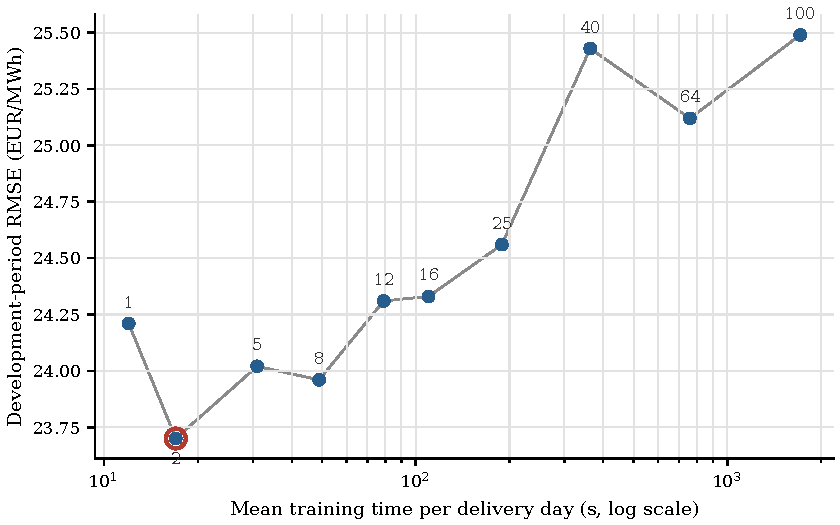
\includegraphics[width=0.72\textwidth]{figures/price_base_cluster_pareto.pdf}
  \caption[Accuracy--runtime frontier of the base price model weather
  clustering.]
  {Development-period RMSE against mean training time per delivery day for the
  base price model, over weather-cluster counts from 1 to 100 at a 70-day
  window. The selected two-cluster representation is highlighted.}
  \label{fig:price_base_cluster_pareto}
\end{figure}

\FloatBarrier

\subsubsection{Reserve-Market Ablation}
\label{app:reserve_ablation}

Table~\ref{tab:reserve_ablation} isolates the effect of the reserve-market
features by comparing each cutoff price model with an otherwise identical model
that excludes the reserve-market covariates, on the same matched panel. Before
the EXAA price is admissible, adding the reserve-market results lowers the RMSE
at every cutoff, by 1.1\% at 09:00, 3.4\% at 10:00, and 2.1\% at 11:00. Only the
10:00 improvement, after the aFRR results enter, is significant on its own, and
it does not remain significant after the Holm correction across the three
pre-EXAA cutoffs. At the 12:00 cutoff, once the EXAA price is admissible, the
reserve-market features no longer help and slightly increase the error, which is
consistent with the EXAA signal absorbing most of the short-horizon price
information. The reserve-market results therefore contribute to the gradual
improvement before 12:00, but their effect cannot be established robustly on
this test period.

\begin{table}[H]
  \centering
  \small
  \caption[Reserve-market ablation for the cutoff price models.]
  {Reserve-market ablation for the cutoff price models. Each row compares a
  cutoff model without reserve-market features against the otherwise identical
  model with them, on the matched test panel from 1~February~2026 to
  31~July~2026 (\(n=17{,}184\)). The \emph{With reserve} \mbox{RMSE} column holds
  the selected cutoff models and matches their RMSE in
  Table~\ref{tab:rq3_cutoff_results}, while the \emph{No reserve} column is the
  counterfactual without reserve-market features. Errors are in EUR/MWh.}
  \label{tab:reserve_ablation}
  \begin{threeparttable}
  \begin{tabular}{@{}llrrrr@{}}
    \toprule
    Cutoff & Reserve products & \multicolumn{2}{c}{RMSE}
      & \(\Delta\)RMSE & \(p_{\mathrm{GW}}\)\tnote{a} \\
    \cmidrule(lr){3-4}
    & & No reserve & With reserve & & \\
    \midrule
    09:00 & FCR & 32.76 & 32.39 & -1.1\% & 0.23 \\
    10:00 & FCR, aFRR & 32.89 & 31.78 & -3.4\% & 0.025 \\
    11:00 & FCR, aFRR, mFRR & 31.46 & 30.81 & -2.1\% & 0.11 \\
    12:00\tnote{b} & FCR, aFRR, mFRR & 27.27 & 27.58 & +1.1\% & --- \\
    \bottomrule
  \end{tabular}
  \begin{tablenotes}[flushleft]
    \footnotesize
    \item[a] One-sided GW p-value, squared-error loss, with against
    without reserve-market features. None remains significant after a Holm
    correction across the three pre-EXAA cutoffs.
    \item[b] Both 12:00 models include the EXAA price. The reserve-market features
    do not improve the forecast, so no p-value is reported.
  \end{tablenotes}
  \end{threeparttable}
\end{table}

\FloatBarrier

\subsubsection{Detailed Feature-Importance Results}
\label{app:feature_details}

The grouped shares in Section~\ref{sec:results_feature_importance} aggregate over
feature groups. A subgroup collects all the per-MTU columns of
one signal, such as the lagged price on day \(d-1\), which enters as a separate
feature for each of the 96 quarter-hours, or the OBTF residual-load forecast.
Tables~\ref{tab:rq2_top_features} and \ref{tab:rq3_top_features} break the feature
groups down one level finer, into these subgroups, for the price forecast with
OBTF load and renewable-generation forecasts \(\hat{P}^{\mathrm{gen}}\) and for the full 12:00 cutoff
model.

Shares use the same normalization as the grouped shares in
Figures~\ref{fig:rq2_feature_importance} and~\ref{fig:rq3_feature_importance}, so
a group with a single subgroup, such as the EXAA price, matches those figures
exactly. Subgroups within a group need not sum to the group share, because
importance is measured as a mean absolute contribution: when two subgroups in the
same group push the forecast in opposite directions on a given prediction, their
effects partly cancel in the group total, so the group's absolute contribution is
smaller than the sum of the subgroups' absolute contributions.

For \(\hat{P}^{\mathrm{gen}}\), the residual-load level is the single largest
subgroup, followed by the previous-day price lag, with the residual-load ramp,
wind, radiation, and the OBTF renewable-generation forecasts contributing further.
For the 12:00 model, the EXAA price subgroup alone accounts for about
two-thirds of the contribution mass, far ahead of the residual-load level, the
previous-day price lag, and the reserve-market results, which confirms the dominance of the late EXAA signal
at the final cutoff. Figure~\ref{fig:rq2_shap_beeswarm} shows the direction of the
leading effects in \(\hat{P}^{\mathrm{gen}}\). Higher recent prices and higher
residual load push the forecast up, while higher wind generation pushes it down,
in the economically expected direction.

\begin{table}[H]
  \centering
  \small
  \caption[Leading feature contributions in the RQ2 price model.]
  {Subgroups with the largest mean absolute SHAP contribution for \(\hat{P}^{\mathrm{gen}}\), combining each signal
  over its MTUs.
  Shares are percentages of the model's total grouped contribution.}
  \label{tab:rq2_top_features}
  \begin{tabular}{@{}llr@{}}
    \toprule
    Subgroup & Group & Share (\%) \\
    \midrule
    Residual load & Residual load & 36.9 \\
    Lagged price (day \(d-1\)) & Price lags & 21.2 \\
    Residual load ramp & Residual load & 9.9 \\
    Wind generation & Renewables & 9.9 \\
    Shortwave diffuse radiation & Raw weather & 6.2 \\
    Wind speed & Raw weather & 5.8 \\
    Shortwave direct radiation & Raw weather & 5.0 \\
    Load forecast & Load & 4.6 \\
    Solar generation & Renewables & 4.5 \\
    Total renewable generation & Renewables & 4.1 \\
    \bottomrule
  \end{tabular}
\end{table}

\begin{table}[H]
  \centering
  \small
  \caption[Leading feature contributions in the 12:00 cutoff model.]
  {Subgroups with the largest mean absolute SHAP contribution for the
  full 12:00 cutoff model, combining each signal over its MTUs.
  Shares are percentages of the model's total grouped contribution.}
  \label{tab:rq3_top_features}
  \begin{tabular}{@{}llr@{}}
    \toprule
    Subgroup & Group & Share (\%) \\
    \midrule
    EXAA price & EXAA & 66.9 \\
    Residual load & Residual load & 6.9 \\
    Lagged price (day \(d-1\)) & Price lags & 6.1 \\
    Reserve market & Reserve & 5.7 \\
    Residual load ramp & Residual load & 3.9 \\
    Wind generation & Renewables & 2.8 \\
    Wind speed & Raw weather & 2.7 \\
    Shortwave diffuse radiation & Raw weather & 1.9 \\
    Total renewable generation & Renewables & 1.7 \\
    Shortwave direct radiation & Raw weather & 1.6 \\
    \bottomrule
  \end{tabular}
\end{table}

\begin{figure}[H]
  \centering
  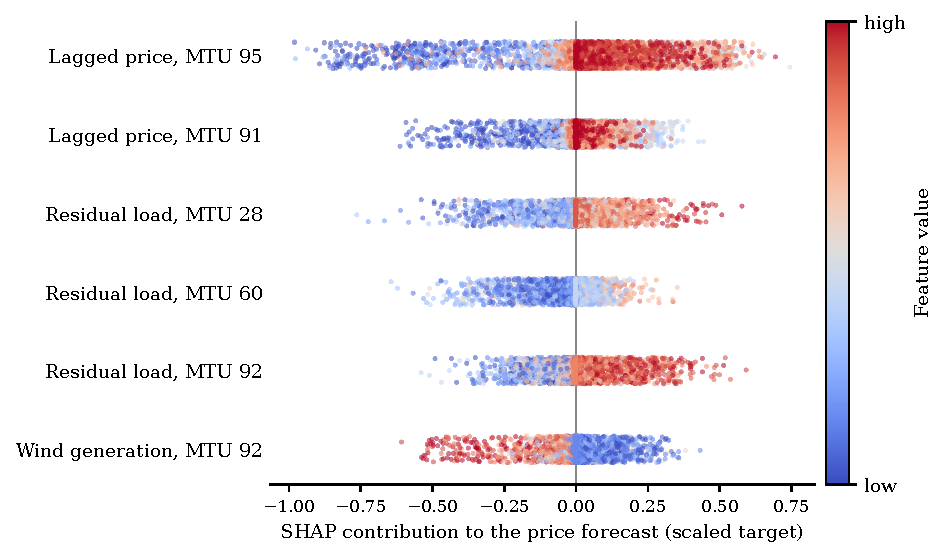
\includegraphics[width=0.82\textwidth]{figures/rq2_shap_beeswarm.pdf}
  \caption[Direction of the leading feature effects in the RQ2 price model.]
  {Direction of the leading feature effects for \(\hat{P}^{\mathrm{gen}}\). Each
  point is one sampled prediction, its horizontal position is the feature's SHAP
  contribution to that forecast, and its color is the feature value from low
  (blue) to high (red). Contributions are on the scaled model target, so only
  their direction and relative magnitude are interpretable.}
  \label{fig:rq2_shap_beeswarm}
\end{figure}

\FloatBarrier
